\section{Introduction}
\label{sec:slam-intro}
This chapter presents the development and evaluation of a LiDAR-inertial SLAM pipeline designed to operate independently of frequent GNSS updates, targeting three core requirements. First, the system must achieve high-fidelity localisation in GNSS-denied or GNSS-degraded scenarios. Second, the SLAM front-end must remain invariant to fluctuating visual appearances, enabling continuous operation across diurnal cycles, varying weather conditions, and seasonal plant growth. Third, as described in \cref{chap:Background}, vineyard and orchard rows form long, symmetric, corridor-like structures that limit the geometric diversity available to scan-matching algorithms, making them susceptible to ambiguity and longitudinal drift, as illustrated in \cref{fig:slam-map-zoomed-out}. The system presented in this chapter is therefore not intended as a general-purpose SLAM solution; it is a specialised architecture targeted at the structural and perceptual characteristics of row-crop environments such as vineyards and orchards. The two primary contributions of this chapter are: (i) a systematic hyperparameter optimisation methodology for tuning LiDAR-inertial SLAM to the specific geometric and operational demands of row-crop environments, and (ii) an extension of the SLAM back-end to incorporate sparse GNSS factors, enabling bounded long-term drift without continuous RTK availability.

\begin{figure}[htbp]
    \centering
    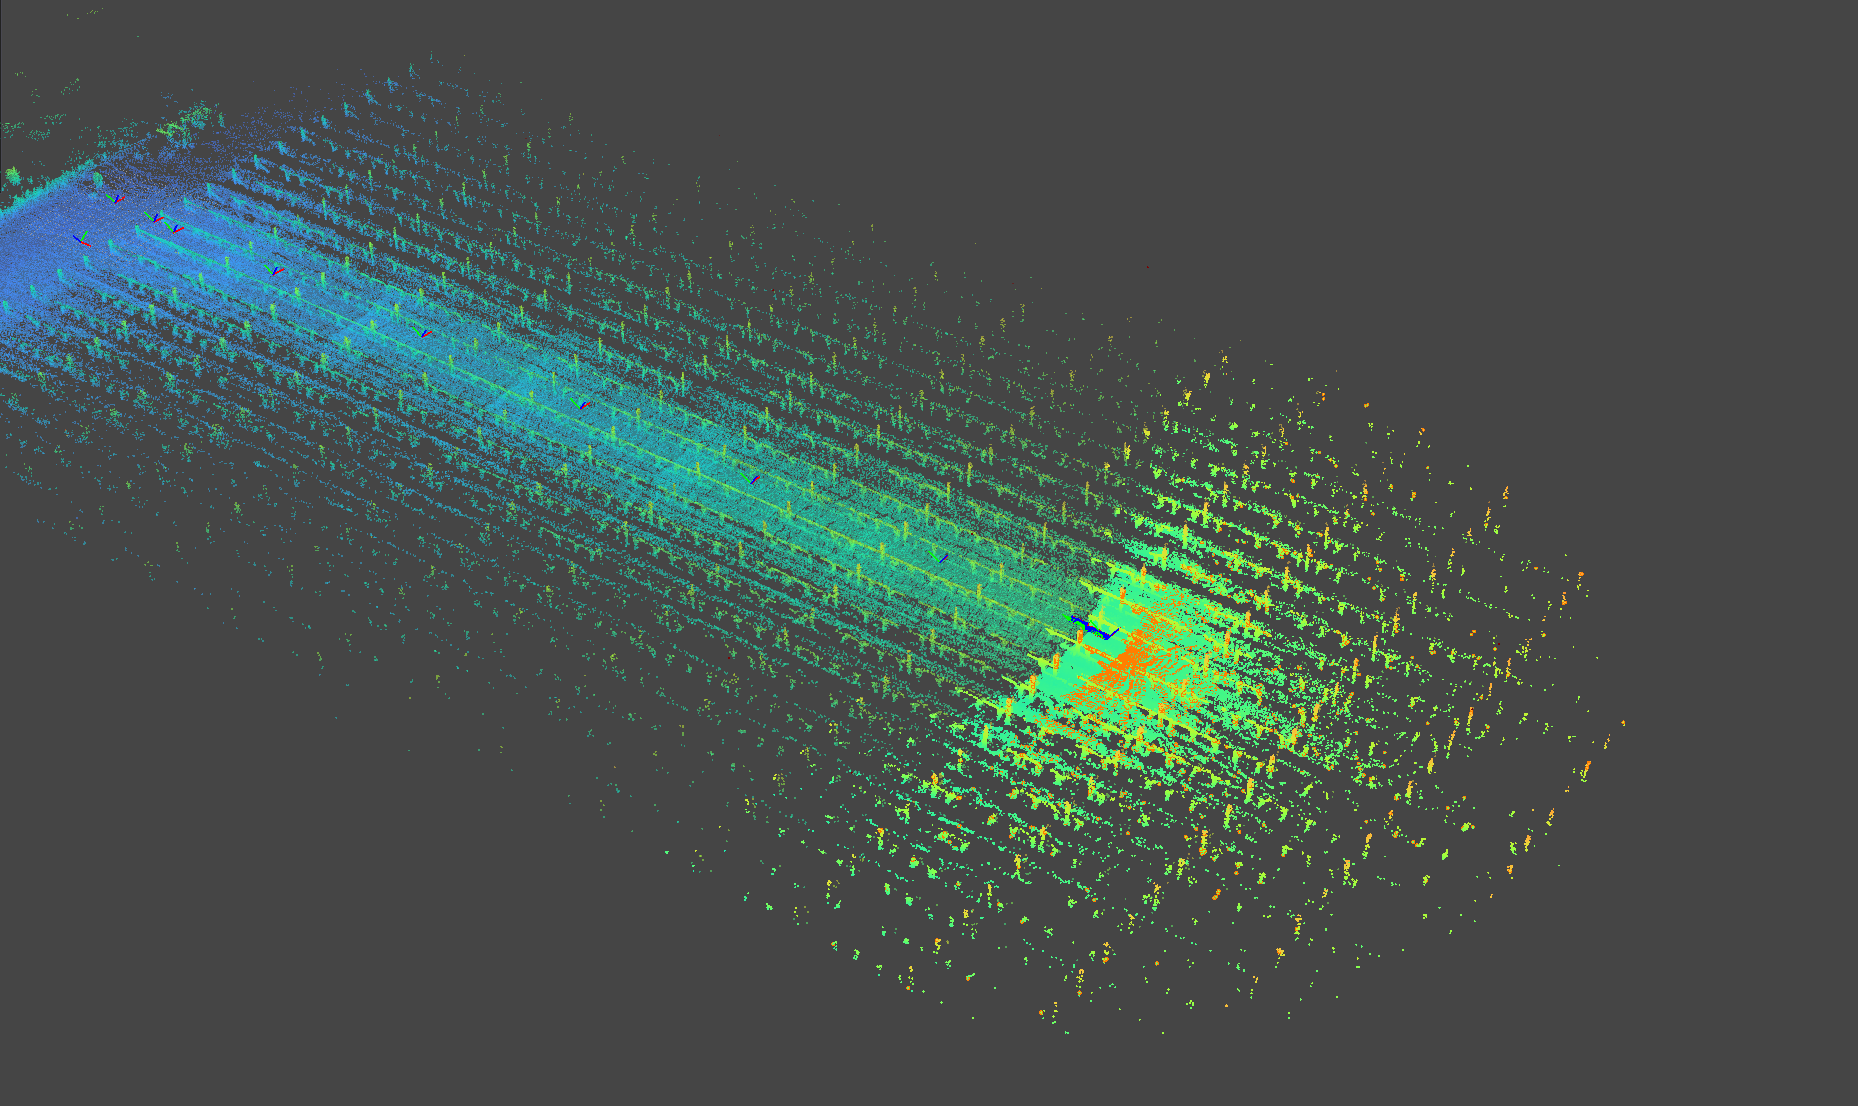
\includegraphics[width=0.85\linewidth]{3-SLAM/3-intro/figures/slam_map_zoomed_out.png}
    \caption{LiDAR point cloud accumulated mid-traversal by the GLIM-GNSS system in the UCVision vineyard (height-coded colouring). The robot is still progressing down a row; the rightmost region of the map remains unvisited.}
    \label{fig:slam-map-zoomed-out}
\end{figure}

\subsection{Motivation}
\label{subsec:slam-motivation}
The necessity for this research stems from the operational limitations of the current UCVision Rover localisation system. Prior iterations of this platform utilised an Extended Kalman Filter (EKF) heavily reliant on Real-Time Kinematic (RTK) GPS data. While precise under open skies, this dependency proved non-viable for robust field operations where tree canopies, topography, and public RTK base station blackouts frequently cause signal multipath or dropout. Adverse weather further compounds this unreliability: heavy precipitation increases tropospheric delay errors \cite{solheimPropagationDelaysGPSSignals1999} and multipath reflections from wet vegetation \cite{nievinskiForwardModelingGPSMultipath2014}, while ionospheric disturbances — which are more frequent during solar weather events and magnetic storms — introduce rapid carrier-phase cycle slips that break the integer ambiguity fix and degrade the RTK solution from centimetre-level fixed accuracy to decimetre-level float accuracy or worse \cite{wielgoszAnalysisNetworkRTKIonospheric2005}. In practice, a significant proportion of field scans conducted with the UCVision Rover were rendered unusable due to the inability to acquire or sustain a consistent RTK fix, causing the localisation system to fail entirely.

Transitioning to a LiDAR-centric SLAM approach, tailored to these agricultural environments, provides three distinct advantages:
\begin{itemize}
	\item \textbf{Reduced GNSS dependence:} By shifting the primary motion estimation to scan-matching and loop closure, the system operates with sub-1\% GNSS factor utilisation, removing the requirement for continuous RTK availability.
	\item \textbf{Corridor robustness:} The architecture presented here specifically addresses the structural challenges of row-crop environments through vineyard-focused parameterisation and sensor fusion suited to row-structured terrain.
	\item \textbf{Downstream utility (design intent):} Beyond localisation, the high-density LiDAR maps generated provide a foundation for additional tasks such as landmark detection (e.g., vine trunks and trellis posts), spatial alignment of Gaussian splats captured from opposing sides of a row, and global registration of data across multiple vineyard bays. These downstream applications are not evaluated in this chapter but motivate the map quality requirements.
\end{itemize}
